\section{Informatique contextuelle}
Au centre des systèmes pervasifs et de l'informatique ubiquitaire, l'informatique contextuelle se fait une part de plus en plus grande. Encore une fois, sa définition a fait l'objet de plusieurs débats au sein de la communauté scientifique. Celle la plus couramment utilisé est : << L'informatique contextuelle (\textit{context-aware computing} a pour but de permettre les équipements de fournir de meilleurs services aux utilisateurs par l'utilisation d'information de contexte >>\cite{Han:contextaware}.

\subsection{Définition et applications}
La définition de contexte a été elle aussi au cœur de nombreux débats. Après analyse des travaux sur le sujet, le rapport de recherche \cite{Dey:context} propose la définition suivante :

\begin{defi}[Contexte]
Un contexte est toute information pouvant être utilisée pour caractériser la situation d'une entité. Cette entité pouvant être une personne, un lieu, ou un objet considéré comme pertinent à l'interaction entre l'utilisateur et l'application, incluant l'utilisateur et l'applications eux-mêmes.
\end{defi}

Il est important de noter sa définition est donc orientée par l'utilisation avant tout qui en est faite. Une donnée quelconque peut être un contexte s'il est utilisé comme tel. Ainsi, il nous faut voir l'ensemble des utilisations de ce contexte. Ces applications visent sept utilisations principales~\cite{Soylu:context} : 
\begin{enumerate}
	\item Sélection et recommandations d'informations ou de services.
	\item Présentation et accès à l'information et aux services.
	\item Recherche d'information ou de service.
	\item Adaptation de l'exécution de processus séquentiels.
	\item Modification et reconfiguration d'applications.
	\item Conseil d'actions semi-automatique.
	\item Allocations de ressources.
\end{enumerate}
\TODO{Est-il nécessaire de fournir des explications ?}

Les thèmes de ces applications sont directement reliés à la supervision car c'est elle qui permet la construction de ce contexte pour ensuite fournir ces types de services de haut-niveau.

\subsection{Modélisation et capture du contexte}
Le modèle utilisé pour créer et manipuler le contexte peut être sous différentes formes : Basé sur des principes d'intelligence artificielle (ontologies, réseau bayésiens), sur le génie logiciel (UML), les bases de données (Entité-Relation) ou d'autres moyens applicatifs (entrées clefs-valeurs). L'UML et l'ER atteignent rapidement leurs limites d'expressivité. Il devient difficile de manipuler les données sémantiques dans le cadre de contextes larges et hétérogènes à cause de leur rigidité. Leurs fonctionnalités permettent d'abstraire une partie du monde ou de la logique pour un usage restreint. Par opposition, les ontologies n'ont pas ces limites par définition. Il est toutefois important de ne pas négliger ces autres modélisations dû à leur efficacité (comme vu dans la section~\ref{sec:rw:supervision:administration}).

\subsubsection{Les ontologies}
Le terme ontologie a d'abord été introduit par la philosophie grecque. Il représente étymologiquement l'étude de l'être. En informatique, il prend cependant une autre dimension. Tel que l'a défini Kalfoglou~\cite{Kalfoglou:ontology}, une ontologie est \textit{une représentation explicite d'une compréhension commune de concepts importants appartenant à un domain d'intérêt}.
Elle permettra donc de capturer et représenter une vue simplifiée d'un domaine à travers des concepts prédéfinis. Cela permet un langage commun et une taxonomie des concepts tout en étant capable de représenter leurs liaisons. Ainsi, il est possible de capturer la sémantique propre des différentes données.

Son expression est simpliste car toute sa structure est orchestrée par des triplets : Objet, Relation, Valeur. Par exemple, \textit{la télévision} \textbf{est située dans} \textit{le salon}. De même, \textit{le salon} \textbf{est une} \textit{pièce}. Toutes les informations sont descriptibles à un niveau concept tout comme à un niveau instance. Les ontologies sont toutefois structuré dans un langage en particulier qui permet de définir les grandes catégories de relations ou d'objets. Plusieurs langages existent mais tous définissent les entités suivantes :
\begin{itemize}
    \item[\textbf{Concepts}] Décrivent les classes et sous-classes de toutes les choses du monde.
    \item[\textbf{Instances}] Ce sont les individus correspondant aux concepts.
    \item[\textbf{Relations}] Permet de lier les concepts et instances entre eux. Une des relations principales est la relation \textit{Est-Un} (\textit{Is-A} en anglais) qui lie une instance à un concept.
    \item[\textbf{Types} de données] Types syntaxiques d'une donnée : entier, chaîne de caractères, booléen.
    \item[\textbf{Valeurs}] Valeur qu'un concept ou instance peut avoir.
\end{itemize}

D'un point de vue expressivité, les ontologies jouissent d'un plus grand pouvoir que les structures telles que les modèles de classes et d'objets d'UML par exemple. Il est toutefois important de noter que cette puissance et cette liberté rend sa manipulation délicate. En effet, il est supposé que toutes les sources de connaissances s'appuient sur des concepts communs. Ceux-ci vont représenter la connaissance du domaine, qui doit se représenter en fonction de son application~\cite{CitationsCharbelpage77}. Il est ainsi important d'être minutieux dans la manipulation de cette structure pour éviter par exemple des duplications de concepts, voire même des conflits de définitions.


\subsubsection{Capture du contexte}
La capture du contexte est la manière de récupérer une information et de la représenter sous la forme choisie lors de la modélisation. Par exemple, un capteur de température pourra insérer un ensemble de triplets pour indiquer qu'à 10h25 le lundi 26 avril, il faisait 25.256ºC sur la source T75896. Cet ensemble de triplet dépendra de la modélisation des concepts qui formeront le contexte. Plusieurs types de captures existent : la capture physique, où les informations sont extraites de l'environnement physique ; la capture logique, où les informations sont issus d'applications ou de services ; et enfin la capture virtuelle où les données sont extraites à partir d'autres informations de contexte.

\subsection{Capacités de traitement}
Un des principal intérêt des structures sémantiques est le pouvoir de raisonnement logique. Le but ici est de pouvoir inférer de nouveaux triplets à partir des connaissances accumulées. Pour cela, il existe plusieurs langages permettant de faire ce type d'inférence. Le plus courant est le langage associé à RDF : \textit{SPARQL}. Ce langage a la particularité d'être aussi expressif que l'algèbre relationnelle~\cite{Angles:sparql}\footnote{Plus exactement, SparQL est équivalent au datalog non-récursif avec négation, ce qui est équivalent à l'algèbre relationnelle.}. Ainsi, il est possible de faire des inférences du premier ordre sur ces données avec une é.

Ces inférences sont de trois types :
\begin{itemize}
 \item L'association directe, à une information bas-niveau est associé une information haut-niveau 
 \item La fusion de contexte, à partir d'un ensemble de données est inféré un nouvel état 
 \item La fission de contexte, à partir d'une donnée est inféré un ensemble d'informations
\end{itemize}

Dans l'informatique contextuelle, il est important de distinguer plusieurs espaces de données~\cite{Padovitz:agent}. 
\begin{itemize}
 \item[\textbf{L'espace de valeur}] Par exemple, pour une personne, son age sera compris entre 0 et 125.
 \item[\textbf{L'espace applicatif}] L'ensemble des données atomiques qui représentent le contexte dit de bas-niveau.
 \item[\textbf{L'espace de situation}] Reflète les situations pouvant être extraits de l'espace applicatif.
\end{itemize}

A un instant donné, il est possible de définir un \textbf{état de contexte} en tant que collection d'attributs de l'espace de contexte. Cet état pourra par la suite, grâce aux opérations présentées, inférer un ensemble de situations. La figure~\ref{rw-supervision-contextreasoning} montre la structure abstraite du raisonnement sur les contextes.
\begin{figure}[ht]
    \centering
    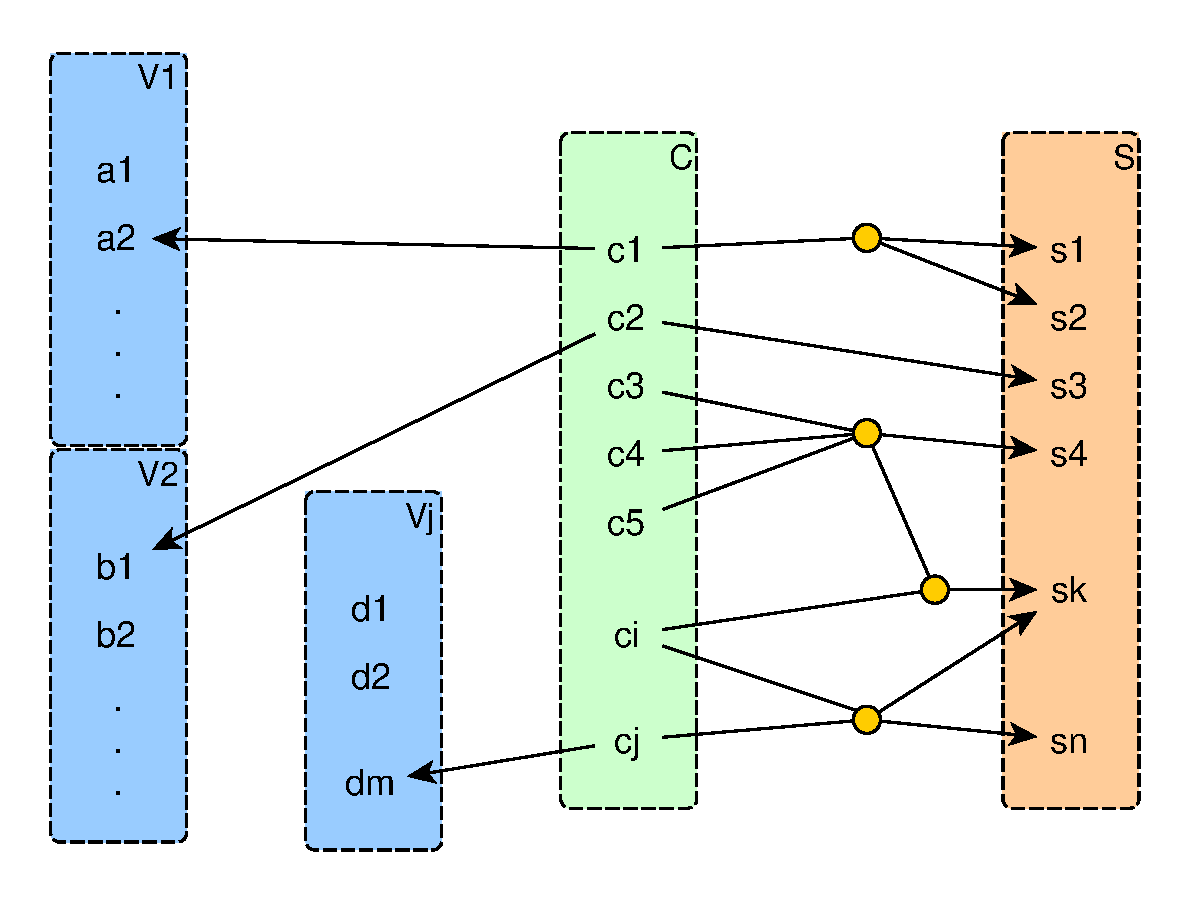
\includegraphics[width=.50\textwidth]{rw-supervision-contextreasoning}
    \caption{Structure abstraite du raisonnement sur contexte. À un élement du contexte $c_i$ est associé une valeur du domaine $V_i$. A partir de l'espace du contexte $C$, on effectue des associations, des fissions ou fusions pour inférer l'espace des situations $S$.}\label{rw-supervision-contextreasoning}
\end{figure}



L'inférence est en relation directe avec les critères de qualités évoqués précédemment. Les critères sur la précision / fiabilités / résolutions introduiront de l'aléa de mesure ainsi les situations inférées ne seront pas certaines. De même les critères sur la confiance et la fraîcheur introduiront des résultats qui devront refléter ces points de vue. Enfin, l'inférence se fait par des règles ou par raisonnements. Les règles définies par diagnostic ou par l'utilisateur ne sont pas tout le temps fiables (par exemple, un diagnostic de pixelisation TV est souvent dû à un problème de lenteur de réseau interne, mais ce peut être du à des dysfonctionnements plus rares du matériels (surchauffe)). Ainsi, nous introduisons une part de probabilités dans ces raisonnements pourtant déterministes a priori.

\subsection{Analyse de systèmes pervasifs existants}
Dans cette partie, nous analyserons des systèmes pervasifs existants. Ceux-ci sont en général très orientés sur la domotique (\textit{Home Automation}) qui est l'environnement de développement le plus courant dans le domaine de l'informatique ubiquitaire.

\subsubsection{DogOnt}
\subsubsection{Amigo}
\subsubsection{MATCH}
\subsubsection{SOCAM}
\subsubsection{Gathor Tech House}
\subsection{Synthèse}
\TODO{Et c'est reparti pour le tableau}